
%(BEGIN_QUESTION)
% Copyright 2006, Tony R. Kuphaldt, released under the Creative Commons Attribution License (v 1.0)
% This means you may do almost anything with this work of mine, so long as you give me proper credit

Fail-safe control system design does not end with the control valve, although it does begin with it.  In order to maximize the safety of the control system in critical applications, the designer should choose a configuration for {\it each instrument in the loop} that leads to the exact same (safest) failure mode.

Closely examine the following loop diagram for a compressor surge control system, designed to open bypass valve FV-42 in the event that differential pressure across the compressor becomes too great and/or flow through the compressor becomes too little.  When valve FV-42 opens, it shunts gas flow from the outlet to the inlet of the compressor, both increasing compressor gas flow and decreasing differential pressure:

$$\includegraphics[width=15.5cm]{i00794x01.eps}$$

Take special note of the up or down arrows next to each instrument's calibrated range in the diagram.  These arrows indicate the {\it action} of the instrument, either direct or reverse.  An up arrow ($\uparrow$) near the instrument indicates direct action: the instrument's output increases as its input increases.  A down arrow ($\downarrow$) near the instrument indicates a reverse-action instrument: one whose output decreases as its input increases.

\vskip 10pt

Perform a series of ``thought experiments'' whereby you analyze the action of the control system (to bypass the compressor or not to bypass the compressor) in the event of {\it any} break in {\it any} cable.  Explain how the system responds in each case, step by step, resulting in the safest condition every time.

\vskip 20pt \vbox{\hrule \hbox{\strut \vrule{} {\bf Suggestions for Socratic discussion} \vrule} \hrule}

\begin{itemize}
\item Explain why the shield conductor of each cable is grounded only at one end, not at both ends.
\item Explain why such ``thought experiments'' are useful techniques for analyzing control systems, and why you as a technician should become comfortable with applying this problem-solving technique on the job.
\end{itemize}

\underbar{file i00794}
%(END_QUESTION)





%(BEGIN_ANSWER)

For every cable break, the system responds by opening FV-42 to bypass the compressor: the safest possible condition.

\vskip 10pt

For your information, compressor surge is a fluid dynamic phenomenon whereby the blades in a non-positive-displacement compressor (e.g. axial or centrifugal vane) ``stall'' just like the wings of an airplane flying too slowly and/or at too great an angle of attack.  When the blades of a compressor stall, they lose ``traction'' on the compressed gas, unloading the mechanical driver (engine, motor, or turbine) and allowing the compressor to gain speed, then the blades will ``un-stall'' and re-load the driver, continuing the cycle.

The following passage is taken from Francis Shinskey's excellent treatise {\it Energy Conservation and Control}, published by Academic Press in 1978, describing compressor surge:

\vskip 10pt {\narrower \noindent \baselineskip5pt

``The most demanding aspect of controlling compressors is surge protection.  The problem lies in being unable to determine with absolute certainty the degree of approach to surge.  Once a compressor begins to surge, it will continue until corrective action is applied, so automatic protection is mandatory.  A small centrifugal compressor may surge several times without damage, but a 100,000-hp axial could require reblading after a single incident.''

\vskip 5pt

``When a compressor begins to surge, the suction flow falls to zero within a few milliseconds, reverses momentarily, and begins to recover in less than a half second.  If the situation is not corrected, the cycle repeats immediately, resulting in a series of thunderclaps less than a second apart.  The sudden fall in suction flow can be detected and used to open a recirculating valve, but not before at least one surge cycle is sustained.  To prevent surge from developing at all requires a control system which skirts the unstable area altogether.''

\par} \vskip 10pt


%(END_ANSWER)





%(BEGIN_NOTES)

Note: the cable shields are grounded at one end only to avoid {\it ground loops}.





\vskip 20pt \vbox{\hrule \hbox{\strut \vrule{} {\bf Virtual Troubleshooting} \vrule} \hrule}

This question is a good candidate for a ``Virtual Troubleshooting'' exercise.  Presenting the diagram to students, you first imagine in your own mind a particular fault in the system.  Then, you present one or more symptoms of that fault (something noticeable by an operator or other user of the system).  Students then propose various diagnostic tests to perform on this system to identify the nature and location of the fault, as though they were technicians trying to troubleshoot the problem.  Your job is to tell them what the result(s) would be for each of the proposed diagnostic tests, documenting those results where all the students can see.

During and after the exercise, it is good to ask students follow-up questions such as:

\begin{itemize}
\item What does the result of the last diagnostic test tell you about the fault?
\item Suppose the results of the last diagnostic test were different.  What then would that result tell you about the fault?
\item Is the last diagnostic test the best one we could do?
\item What would be the ideal order of tests, to diagnose the problem in as few steps as possible?
\end{itemize}

%INDEX% Control, fail safe: choosing best failure modes for all loop components
%INDEX% Documentation, loop diagram: compressor surge control
%INDEX% Final Control Elements, valve: fail safe
%INDEX% Process: compressor surge control

%(END_NOTES)


